\section{Mitigating the Latency of programming network state}

\iffalse

\aditya{the following three may have to go earlier} 

Recall the 4 steps O1--O4 taken by a switch to process \flowmod
messages described in \S\ref{s:motivation}. Although TCAMs support far
lower update rates than reads, updates (step O4) are still quite fast:
typically each rule write takes well under a fraction of a
millisecond. However, the non-trivial latencies we observe when
inserting a burst of equal priority rules (where we see each rule
insertion taking >2ms on average) indicate that the impact of steps O1
and O2 appear to be significant. Our conversations with switch vendors
indicate that software implementations have gotten more
optimized\footnote{Early implementations of OpenFlow switches were far
  worse; e.g., the SDK to the underlying chip in first generation
  OpenFlow switches was never meant to be used to quickly add ACLs to
  the chip. Rule insert latencies were 10ms or even higher as a
  result}, but they appear to still be quite far from optimal.

Our measurements with rules having priorities show that step O3 has a
significant impact on latency. Even if switch software implementations
improve, the latency imposed due to the memory chip and its SDK are
likely to remain significant.

%Finally, we note that depending on the switch implementation, it is likely that
%there may be additional steps involved whose latency impact is not captured by
%our work. 

Will software implementations improve in the near future such that
rule update rates improve and latencies in steps 1 and 2 disappear? We
don't believe so: switch vendors will not put in the software effort
to get update rates up unless they see them as a
differentiator. Customers continue to make purchase decisions mostly
based on line speeds and perhaps flow table sizes, and hence they will
not get high update rates.  \aditya{the above text can go toward end
  of section 3, or it can be taken out completely if it seems like it
  is underplaying our contributions.}.

\fi

% To some extent, this has been optimized in recent switches.

% When a switch receive multiple rules to install in a batch, it may undertake additional steps. These include: 1.1) Commonly used memories, e.g., TCAMs, support update/writes at a much slower rate than reads.

% Our measurements indicate that while 1.1 does not impact latencies, 2.1 and 2.2 do have a telling effect. 

\iffalse
We describe three Mazu modules for overcoming outbound
latencies. 
% The central requirement for our techniques is that they
% must be applicable to a variety of management of applications as
% generically as possible. This allows our techniques to be implemented
% as a library that application can freely leverage to manage the impact
% of outbound delays without significant changes to application logic.
% The key insight underlying all our approaches is to modulate the input 
% provided to a switch such that rule installation latency is minimized 
% given the underlying latency causes.
Our approaches deal mainly with rule insertions. To
handle rule deletions and modifications, we leverage the
following key ideas based on our measurement results: 

1. {\em Avoid
  deleting rules:} Rule deletions are expensive across
all the platforms we measured. Thus, {\em we try to avoid rule deletion}.
Instead, we simply let them time out (and insert higher priority rules
to supersede them as needed). 

2. {\em
  Avoid modifying rules for Broadcom}: Our measurements with both
Broadcom switches showed that modifying a rule is more expensive than
inserting a new rule.
% (the former incurs the cost of potentially
% reshuffling the entire existing set of rules at the switch, whereas
% the latter only displaces lower priority rules)
Therefore, we {\em always insert} a new rule $R'$ for a flow at a switch instead
of modifying the existing $R$ to $R'$. We ensure $R'$ is of higher priority than $R$
but lower priority than any $R''$ that overlaps with $R'$ and is
higher priority than $R$. We simply let $R$ expire (similar to
above). A nice side-effect of this is that rule priorities
generally ``stay high'', resulting in lower rule displacements from
future insertions compared to modifying rules (as only higher priority
rules can cause displacements in Broadcom). For the Intel switch,
%and insertion costs are identical, 
modification latency is small and independent of rule priorities in the flow table, so
no such provision needs to be made.


\fi
% \subsection{Overview}

% We propose three techniques
% that can be applied individually or in tandem. These are shown in Figure XXX.


% It helps mitigate the unknown
% impact of additional steps a switch may take. Its
% effectiveness can be enhanced by using it in combination with the
% rest of the techniques. \aditya{may need to reword this}  

% a set of application-dependent techniques 

% Outbound delay are impacted by queuing, TCAM reordering and switch firmware
% processing. To avoid excessive queuing delay, the controller can avoid picking
% switches with a large number of outstanding flow\_mod messages. TCAM reordering
% is affected by the rule priorities. To avoid excessive reording delay, we can
% leverage multiple tables in a single switch or multiple switches so that each
% TCAM table will only be installed with rules that have a small number of
% priorities. Due to the asynchrony between the controller state and switch state
% and the blackbox nature of switch firmware, some portion of outbound delay will
% not be predictable. We handle this by setting up multiple paths in parallel.

\subsection{Flow Engineering}
\label{s:floweng}

\begin{figure}
\centering
%\begin{minipage}{.45\textwidth}
  \centering
  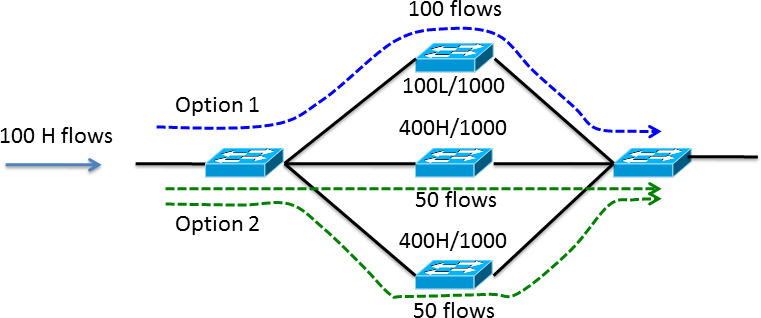
\includegraphics[width=3.2in]{figs/flow_eng.PNG} \compactcaption{Flow 
engineering example, assuming Broadcom. NL = “N” low priority rules; NH 
= “H” high priority rules; capacity = 1000 rules. Ingress and egress 
tables are empty} 
\label{fig:flow_eng} \end{figure}

SDN applications typically compute paths between various network
locations that meet some global objective pertaining to
performance or security. A common issue considered in most prior works
on such applications is to deal with limited switch table sizes, by
picking routes that obey or optimize table space
constraints~\cite{swan,simple, minlanvcrib}. Unfortunately,
these techniques do not provide sufficient control over outbound
delay. 

\minisection{Minimize maximum flow table occupancy is very suboptimal} 
For example, consider a simple setting where there are three candidate
paths between a pair of nodes as shown in Figure~\ref{fig:flow_eng}.
Each path has one Broadcom switch. The switch on the first path
has 100 rules of low priority L, whereas the switches on the second
and third paths each have 400 rules of high priority H. Suppose that a
hypothetical traffic engineering application has 100 flows of priority
H to allocate to these paths, and each path is equally preferable
for a flow.  Existing techniques for table space management would
assign all flows to the first path to minimize maximum flow table occupancy; but
our measurements for Broadcom 
show that {\em each} of these 100 rules will displace
all the 100 low priority rules in the TCAM, resulting in high
latencies! Allocating 50 flows each on the
latter two paths instead results in no rule displacement, and the number of
rules installed per path will be smaller. Thus, when the flows are installed in
parallel across the latter two paths, this results in significant reduction in
installation latency. Based on Figure~\ref{fig:burst-completion-time}, it is about 200 ms
vs 2 seconds, a 10X difference. 
%Intel switches have similar issues, but for other priority patterns.
%li: yes, according Marina's information. Low priority rule displaces high
%priority rule depending on their location.
%\aditya{check intel claim}

The goal of flow engineering is to select paths across the network
such that installation delay is minimized. The key insight we use is
the following: in general, there are many possible sets of paths
$\{\mathcal{P}^i_{obj}\}_i$ in a network that optimize an SDN
application's objectives, e.g., optimal capacity and latency. From
this, flow engineering selects the set
$\mathcal{P}^{displace}_{obj,tbl\_sz}$ that minimizes the aggregate
impact of both rule displacement in TCAM as well as the number of rules
installed at any switch, while obeying table space constraints.
% maximum number of rules installed at any
% switch; thus, we spread rule update load {\em laterally}, helping
% improve outbound latencies.
%
$\mathcal{P}^{displace}_{obj,tbl\_sz}$ can be computed by running a
two step optimization, where the first step computes the value of the
network's objective function, but not the actual routes to use, and
the second step computes routes that minimize the aggregate effect of
rule displacement and the number of rules to be inserted at any switch.
The detailed optimization formulation is a large integer linear
program (omitted for brevity) and hence inefficient to solve. Below,
we discuss a simplifying heuristic in the context of a traffic
engineering application.

We represent the network as a graph \textit{G
  = (V,E)}, where each node is a switch (or a PoP) and each edge is a
physical link (or virtual tunnel). Given a traffic matrix $M$, the
application attempts to route it such that the average link
utilization is within some bound; the heuristic can be easily extended
to accommodate other objectives.
% Our goal to compute routes such that the
% objective is maximized as well as the cost of installing the necessary
% rules at switches is minimized. 
%Our heuristic works by exploring for each source-destination pair
For each source-destination pair we see,
whether a path can accommodate both its demand, and the path setup latency  
%imposed by routing the pair across the path's switches 
is within some bound. If either is violated, we try the next
candidate path.

More precisely, suppose we want to bound the maximum cost of
installing rules at any switch by some $C$. We start by selecting some
low value for $C$. We assume that we have computed $K$ candidate equal cost
paths for each $(u,v) \in V$. Suppose the priority of the $(u,v)$ flow
is $Pri(u,v)$ at every switch in the network (this is
typically set by the operator).

We sort the traffic demands in decreasing order and
iterate through them. For each $(u,v)$ in the sorted order, we
consider the corresponding $K$ equal cost paths in decreasing order
of available capacity; let $P^{1\ldots K}_{(u,v)}$ be the sorted order. 

If the demand $d_{uv}$ can be satisfied by the path $P^{1}_{(u,v)}$ within
the utilization bound, then we compute whether installing the $(u,v)$ path
violates the rule installation latency bound or not. We do this by modeling
the per-switch latency, as well as maximum latency on the path:

\minisection{Per-switch latency}
% Recall that we always install new rules,
%and never do rule modifications and deletions. 
%\aditya{the previous sentence may have to go}
% In doing this, an issue to consider is whether the rule for
% $(u,v)$ at $s$ is modifying an existing forwarding rule for $(u,v)$ at
% $s$ (this would happen if $(u,v)$ was being routed through $s$ before,
% but the next hop from $s$ has now changed) or it is a new rule being
% inserted (this happens if $(u,v)$ was never routed via $s$ before).
% However, recall that our measurements show that modifying a rule is
% much more expensive than inserting a new rule (the former incurs the
% cost of potentially reshuffling the entire existing set of rules at
% the switch, whereas the latter only displaces lower priority rules).
% Therefore, we {\em always insert} a new rule for $(u,v)$, ensuring
% that the rule is of higher priority than the existing rule for $(u,v)$
% in $s$ (if any). 
Given our measurement results, for every switch $s \in P^{1}_{(u,v)}$, we can
model the latency at $s$ due to routing $(u,v)$ as $L_s = \max(a, (b +c *
Disp_s(Pri(u,v))))$. Here, $Disp_s(Pri(u,v))$ is the number of rules
at $s$ that will be displaced by the rule for $(u,v)$.
%% the following discussion is not very useful, it seems 
%For the Broadcom switch, this is the number of rules of priority {\em lower}  than $Pri(u,v)$, whereas for the Intel switch
%$Disp_s(Pri(u,v))$ is the number of rules of priority \emph{higher} than
%$Pri(u,v)$ divided by 300. 
%This is a conservative estimate assuming all rules
%are packed in increasing priority of slices (\S\ref{s:meas_insert}).
%\aditya{check intel claim} 
%$Disp_s(Pri(u,v))$ can be easily tracked by the SDN
%controller. In the above, 
$a$, $b$ ad $c$ are constants derived from switch
measurements. This model essentially says that if the current rule
does not displace any rules from $s$'s existing table, then it incurs
a fixed cost of $a$; otherwise, it incurs the cost given by $b +c *
Disp_s(Pri(u,v))$. The fixed cost $a$ is the insertion delay without any TCAM
ordering. 

%$a$ is the same whether it is modification or insertion for Intel. For
%Broadcom, since we avoided modification, it represents insertion delay without
%TCAM displacement. 
%\aditya{refer back to the model from
%  the measurement section}

\minisection{Maximum installation latency} \fixme{why not Minimizing?} Now, $\forall s \in P^{1}_{(u,v)}$
, we check if $L_s + CurrentL_s \le C$, where $CurrentL_s$ is the
current running total cost of installing the rules at $s$, accumulated
from source-destination pairs considered prior to $(u,v)$ in our
iterative approach.

If this inequality is satisfied, we assign $(u,v)$ to the path
$P^{1}_{(u,v)}$ and move to the next source-destination pair. If not,
meaning that installing the $(u,v)$ route on this path violates the
maximum cost bound $C$ for some switch on the path, then we move to
the next candidate path for $(u,v)$, i.e., $P^{2}_{(u,v)}$ and
repeat the same as above.

If after iterating through all $(u,v)$ pairs once, the traffic matrix
cannot be allocated, then we increase $C$ and start over again.
Alternately, we could do a simple binary search on $C$. 
%li: no space for that.
%\aditya{do we need pseudocode?}

%\aditya{assumption: we have a small number of rules we are adding.
%  otherwise, if we can confirm that the decreasing priority weirdness
%  does not apply for all table occupancies, then we should use that}
%\aditya{seems like bcm is buggy so we may not need the above
%  assumption}

% We assign each edge a cost that is the reciprocal of its current available capacity, and find the 
% minimum cost path for the traffic demand. For finding the minimum cost path, we consider precomputed K equal hop length paths, and find
% the path which gives the minimum cost. As we assign a path for a particular traffic demand, 
% we reassign the cost by decreasing the current capacity by the traffic demand for each edge belonging to the
% min-cost path. The idea is that edges which are more highly utilized will get a higher cost value and so the min-cost path for remaining 
% traffic demands will prefer the edges which are lightly utilized. This way, 
% we minimize the maximum load. We analyze the runtime complexity of the algorithm. 

% 
\begin{table}
\begin{scriptsize}
\begin{tabular}{c|l}
Notation & Meaning \\
\hline
$S$ & Set of all switches
\\$S_{ToR}$ & Set of all ToR switches
\\$\tau_{u}$ & Maximum number of flow entries in the switch $u \forall u \in S$
\\$E$ & Set of all physical links (between two adjacent devices)
\\$C_e$ & capacity of individual links $\forall e \in E$
\\$F_{uv}$ & set of all flows from $u$ to $v$ where $u,v \in S$
\\$P_{uv}$ & Set of paths from device $u$ to device $v$
\\$K _{uv}$ & Number of paths from device $u$ to $v$ where $u,v \in S$ 
\\$P^k _{uv}$ & Set of links of $k^{th}$ path from device $u$ to $v$ where $u,v \in S$
\\$T ^f _{uv}$ & Traffic volume from $u$ to $v$ of flow $f$ where $u,v \in S$
\\$util$ & maximum link utilization
\\$I ^{fk} _{uv}$ & Indicator variable denoting that flow $f$ from $u$ to $v$  takes the $k^{th}$ path.
\\$cost$ & maximum cost of rule installation at any switch
\\$M$ & priority of all new rules being inserted
\\$L_s(M)$ & number of rules at switch $s$ of priority lower than $M$
\\ $a$ & cost of installing a rule it has same priority as rules in table
\\ $b$ & constant factor used in modeling rule displacement cost.
\end{tabular}
\label{tab:notation1}
\caption{Notation used in flow engineering formulation.}
\end{scriptsize}
\end{table}

We explain how flow engineering works for simple traffic engineering SDN
application. We represent
the network as a graph \textit{G
  = (V,E)}, where each node is a switch (or a PoP) and each edge is a physical link (or virtual tunnel). Given a traffic matrix, the application attempts to route it such that the maximum link utilization is minimized. Upon computing routes, the application determines the rules to be installed at individual switches. 

For simplicity, we assume that all the rules to be inserted are of the same priority $M$.  We also assume that the control application knows how many rules in each switch have priority lower than $M$, i.e., $L_s(M)$. This can be easily tracked based on history of rule insertions. The notation we use is shown in Table~\ref{tab:notation1}.


{\bf Step 1 - Network Objective:} In the first step we minimize the
maximum link utilization. Let $T ^f _{uv}$ be the traffic volume
 of flow \textit{f} between $(u,v)$, $P^k _{uv}$ be the set of links on
the $k^{th}$ path between (\textit{u,v}). We use a
binary indicator variable $I ^{fk} _{uv}$ to show whether the flow $f$
is on path $k$ or not.  $K _{uv}$ denotes the number of equal hop
length paths between $(u,v)$. 

We have the following capacity constraint: 

% Following are our two
% constraints. First, The total traffic volume from an edge should not
% exceed its $C_e$ times the link utilization limit, $util$. 

\begin{scriptsize}	
\begin{equation*}
    \sum _{u,v \in S_{ToR},~f \in F_{uv},~k  \in P_{uv}~s.t.~e \in P^k _{uv}} T ^f _{uv} *  I^{fk}_{uv} \leq util \times C_e 
\end{equation*}
\end{scriptsize}	
	
The following ensures each flow $f$ takes a single path:	

\begin{equation*}
    \sum _{k  \in P_{uv}} I^{fk}_{uv} = 1 ,\quad \quad \forall u,v \in S_{ToR},~ f \in F_{uv}
\end{equation*}
 
The objective is to minimize the \textit{util}. Note that we do not
compute paths in this step, just the value of the objective function;
suppose the optimal value is $util^*$.

{\bf Step 2 - New Rule Objective:} In second step, we select routes
so as to minimize the rule installation latencies at any
switch. We allow some slack wrt meeting the utilization objective; denote it by
$\delta$. While the second constraint above remains, the capacity
constraint changes to:
 
% First,  traffic traversing from an edge $e$ does not exceed the $C_e$ multipled by 1 $+$ $\delta$ times the $util^*$. $util^*$ is the maximum link utilization we got from the step 1, and  $\delta$ defines an upper limit on maximum link utilization.

\begin{scriptsize}
\begin{equation*}
    \sum _{u,v \in S_{ToR},~f \in F_{uv},~k  \in P_{uv}~s.t.~e \in P^k _{uv}} T ^f _{uv} *  I^{fk}_{uv} \leq (1 + \delta) \times util^* \times C_e 
\end{equation*}
\end{scriptsize}

% We have a similar constraint as above for   Second constraint is same as step 1.\\
  
% \begin{equation*}
%       \sum _{k  \in P_{uv}} I^{fk}_{uv} = 1 ,\quad \quad \forall u,v \in S_{ToR},~ f \in F_{uv}
% \end{equation*}
 % \begin{alignat*}{2}
  %                     & latency = a * entries + c \\
   %                    \text{   where }a \text{ and }c\text{ are constant}\\ 
  %\end{alignat*}

When a rule installed at a switch cause existing lower priority rules to be displaced, we incur a cost that grows linearly with the number of displaced rules, i.e., $b * L_s(M)$, where $b$ is a constant. This cost adds up linearly when a burst of rules is installed. When the burst of rules installed all have the same priority as rules already in the table, we incur a smaller fixed cost per rule, denoted by $a$. Based on this, we track the total cost of rule installation at a switch as follows:
%  for each rule installed at the switch, we incur a cost of we incur a co
% here, we assign a weight ``$a$'' to the number of rules installed and a weight ``$b$'' to the number of rules that need rearrangement:
\aditya{need to make sure we have justification for
  this linear function. provide constants based on measurements.}

\begin{scriptsize}
\begin{equation*}
                       \sum_{u,v \in S_{ToR}, ~f \in F_{uv}, ~k \in
                         P_{uv} ~s.t.~ s\in P^k_{uv} } max(a, b * L_s(M)) I^{fk}_{uv}  +
                       \leq cost \quad \quad \forall s \in S
\end{equation*}
\end{scriptsize}

The objective is to minimize $cost$.   
  



% This can be viewed as solving the following two optimization problems
% in sequence:

% \[
% \begin{array}{lll}
% \text{Problem 1:} & \text{optimize} & NetworkObjective \\
% & \text{subject to} & RuleCapacities \\
% \end{array}
% \]

% \[
% \begin{array}{lll} 
% \text{Problem 2:} & \text{optimize} & NewRuleObjective \\
% & \text{subject to} & NetworkObjective \text{, and, } \\
% & & RuleCapacities
% \end{array}
% \]

% Here $NetworkObjective$ is the SDN application's network wide
% objective function, such as maximum link utilization, $RuleCapacities$
% represent switch table capacities in the network, and
% $NewRuleObjective$ an objective function pertaining to new rules
% inserted at any switch, such as the maximum number of such rules. The
% first optimization problem simply computes the value of the objective
% function, e.g. the maximum link utilization, subject to switch table
% capacity constraints; no actual paths are computed. The second
% optimization problem uses this value as a constraint to compute
% $P^{flowmod}_{obj,tablesize}$.

\minisection{Comments} Because the paths are computed by the SDN application, flow
engineering will necessarily have to be implemented within the
application. 
Flow engineering does not apply to scenarios where route updates are
confined to just one location, presenting no opportunity to spread
update load laterally. One such example is MicroTE~\cite{microte} (\S\ref{sec-motivation}),
where changes in traffic demands are accommodated by altering rules
at the source ToR to reallocate ToR-to-ToR flows across different
tunnels.

\iffalse
{\bf Interaction with Update Semantics:}
Flow engineering has to be designed carefully when
management applications are trying to realize various consistency
properties for their updates~\cite{mahajan13:hotnets}. We explain
using examples below.

If updates of network state from ``old'' to ``new'' are not
orchestrated carefully, a variety of consistency issues can arise:
e.g., there may be forwarding loops, or packets may be forwarded
inconsistently (using old state some times and new state at other
times) at different network hops. Both issues are transient, and flow
engineering (as well as the rule offloading and priority ordering
techniques we describe below) can reduce the duration of such loops
by bounding the time that any network switch spends updating
its state.

In practice, some network operators may want to ensure some semantics
for their updates. One example is packet
coherence~\cite{mahajan13:hotnets}, which means
a packet should see consistent state (always old, or always new) as it
traverses the network. This can be achieved using global version
numbers and one-shot updates~\cite{consistentupdates}: (a) new
forwarding state is added to the core of the network, keeping older
state around; (b) the edge is updated to use the new state only when
all core switches confirm the installation of the new state; prior to
this all forwarding happens using old state; (c) old state is removed
from the network only when there are no more packets forwarded using
it. Flow engineering as formulated above directly helps in this case
by speeding up step (a). 

Consider another example semantics, loop freedom; this can be achieved
by ensuring that switches downstream on a new forwarding path are
updated, and their new state used for forwarding, before those
upstream~\cite{mahajan13:hotnets}. In this case, naively applying flow
engineering as specified above may hurt: because it may increase the
number of switches and paths being updated it may correspondingly
increase the aggregate number of ``dependencies'' to track amongst
different switches' updates, slowing down loop-free updates.
Furthermore, spreading of updates across multiple paths can also
introduce dependency cycles; expensive mechanisms are necessary to
break these cycles~\cite{mahajan13:hotnets}. which further slow down
the update. Thus, the total latency of doing a loop-free update can be
significantly higher with naive flow engineering.

We must therefore design appropriate flow engineering schemes for
different update protocols. We leave a full exploration of this issue
for future work. Where the issue arise, we assume the network is using
one-shot updates.

\aditya{lead out}

\fi

%\subsubsection{MicroTE}

% LocalWords:  Broadcom SDN TCAM rearrangment tbl sz PoP Pri uv Disp CurrentL
% LocalWords:  MicroTE ToR

\subsection{Rule Offload}
\label{s:offload}

\begin{figure}
\centering
%\begin{minipage}{.45\textwidth}
  \centering
  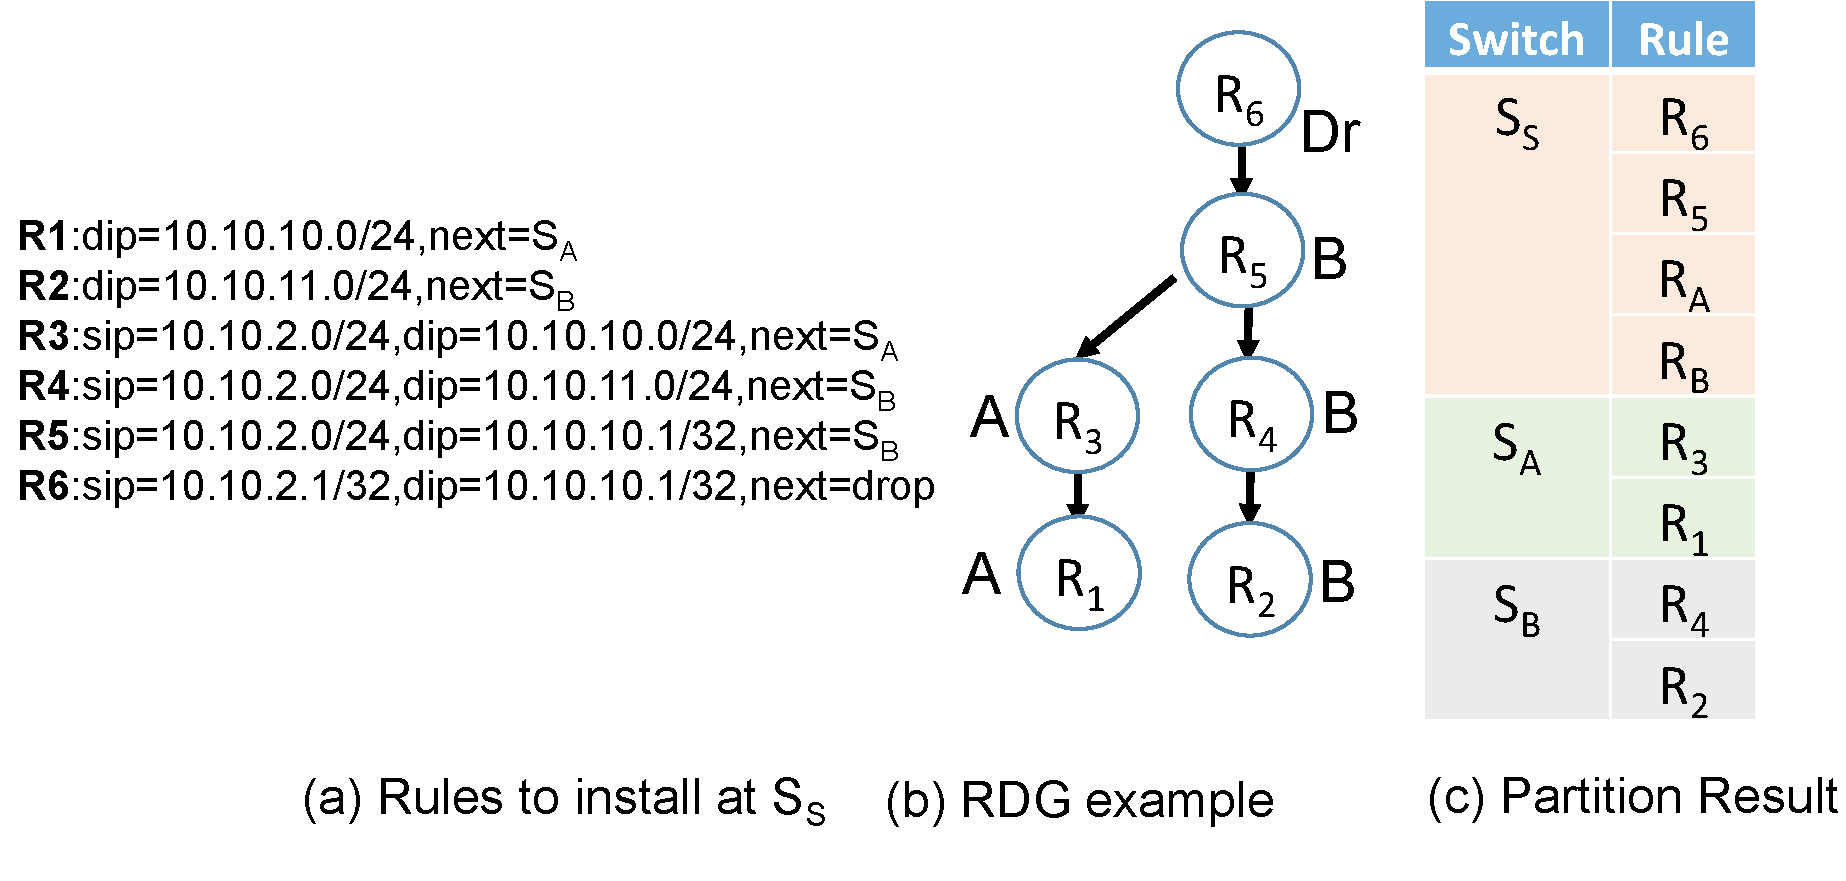
\includegraphics[width=3.0in]{figs/Rule-Offload2.pdf}
\compactcaption{Rule offloading example}
\label{fig:rule-offload}
\end{figure}

%\aditya{LI: this section does not talk about differences wrt difane, vcrib. li, can you fix?}
%\aditya{LI: we should also talk about encapsulation on the core router}

Rule offloading applies particularly to networks where tunnels are
used, e.g., cellular networks (\S\ref{sec-motivation}), carrier networks
that rely on label-switching, data centers using VXLAN
%~\cite{xxx} \aditya{check this} 
and inter-DC WAN networks such as those considered
in~\cite{swan,b4}. In such networks, SDN applications
control the tunnel end-points to setup overlay paths. Compared to the rate of
changes at these tunnel end-points, the underlay, which may also be
run using an SDN, maintains much smaller forwarding state, and
observes much less churn in forwarding state. {\em Our approach
  leverages these attributes of switches in the underlay to offload to
  them rules that would otherwise be installed at the tunnel end
  points.} 

Thus, we wish to partition rules to be installed into a switch into
subsets that can be installed at downstream switches, with the appropriate
default rules added at upstream switches. If the original number of rules is $N$
and no partition (together with default rules) has more than $H$ rules, then we can
reduce rule installation latency by a factor of $\frac{N}{H}$ by updating the
partitions in parallel. 

The main idea in our algorithm is to recursively partition the rules into a
number of child partitions. Since we offload to next hop switches, each
partition has an associated next hop. Rules in
the same partition all go to the same next hop.   
%Actions of rules in a child partition go to the same
%next hop. \aditya{prev sentence does not parse} 
The partition algorithm ensures that there is no dependency among child
partitions. For each partition, we also compute default rules to
direct packets to that partition. The objective is to maximize the number of
rules that can be offloaded minus the number of default rules introduced. 

%li: do not want to disrupt the flow by adding DIFANE; they can read that in
%related work!
%decided the delete the following
\iffalse
Different from~\cite{minlanvcrib}'s goal of reducing computational
load of host hypervisor, our goal in rule offloading is to reduce path
setup latency by enabling fast parallel execution of updates. Also, per
source rule offloading is considered in~\cite{minlanvcrib}. In
contrast, we offload by grouping the next hop of rule actions to
increase offloading opportunities. 
\fi

\fixme{re-present rule offloading}

Before calculating the child partitions, 
we first represent the rules to be installed at the tunnel 
end-point as a rule dependency graph (RDG).  
In a RDG, a node denotes a rule, an edge represents 
the dependency between two rules and the label for 
each node represents the action (or next hop) of the rule. 
%\li{add two simple examples: one for a two-node topology, one for a three-node
%star topology }
We illustrate this using an example in
Figure~\ref{fig:rule-offload}. Figure~\ref{fig:rule-offload}(a) shows the 
topology. Suppose we need to install six rules $R_1$, $R_2$,$\cdots$,$R_6$ to
switch $S_1$. The rule dependency graph is shown in Figure~\ref{fig:rule-offload}(b).
%li: add how to handle rules in table
%If there are rule entries in the flow table, the dependency graph will include
%those rules. 
For example, there is an edge from $R_3$ to
$R_1$. This means that the two rules overlap. When a packet matches both rules,
$R_3$ takes precedence. The labels $A$ and $B$ denote the next hop of the
rules' action. If a rule's action is to send through a tunnel, the label will be
the next hop of the tunnel path, not the tunnel destination.  If a rule's action
is deny, for simplicity, it will not be offloaded. The pseudo code is 
described in Algorithm~\ref{alg:partition}. The time complexity of this algorithm is 
 $\mathcal{O}$($\abs{V}$+$\abs{E}$), where $V$ and $E$ are the 
vertex and edges of rule dependency graph $G$. 
%we can handle the rule depending on the policy and the flow space
%matching it. If it 
%depending on policies, the rule can be skipped in the offloading
%algorithm or can be assigned any next hop. 
%\aditya{this seems wrong; deny rules should apply to *all* paths?} 
%It will be easy to handle deny
%rules. For simplicity, we only consider accept rules. 

\begin{algorithm}
 \KwData{$G$: RDG with nodes annotated with next hop label, 
	$H$: a bound of rule count for core switches,
	$H_{core}$: the maximum number of rules any edge switch 
           can offload to a core switch}
 \KwResult{$P$: partition set for next hops, initially empty}
  \tcc{traverse reverse edges}
  %$N$ = min($H$, $H\_core$)\;
  $G'$ = reverse($G$)\; 
 \While{BFS from leaf node of $G'$}{
  \tcc{$R$ is the current node}
  $i$ = label($R$)\;
  \uIf{$R$ depends on no other rules}{
	 \uIf{rule count of $P_i > H_{core}$ \em{or} core switch $i$'s
	 total rule count $>H$} {
		pin $R$ to $P_{root}$\;
         }
         \Else{
   	       include $R$ in partition $P_i$;\
	 }
   }
   \tcc{$R$ depends on rules with more than one distinct label}
   \Else{
       pin $R$ to $P_{root}$\;
   }
 }
 \caption{Rule Partition}
 \label{alg:partition}
\end{algorithm}

The algorithm starts from the leaf nodes (rules $R$ such that there is no $R'$ with
$R \rightarrow R'$). All of them with the same next hop are placed in one
partition. 
The outcome of the above routine is an allocation of rules to the root
(ingress switch), and to its next hops.
%try to make the following simpler
\iffalse
In the example, we have two next hops $S_3$ and $S_2$ through port A
and B respectively. We have two leaf rules $R_1$ and $R_2$. $R_1$'s next hop is
$S_3$ and $R_2$'s next hop is $S_2$. $R_1$ will be in partition 1 and $R_2$ will
be in partition 2. Since we have $R_3 \rightarrow R_1$ and $R_3$'s next hop is
the same as $R_1$ (which is $S_3$ through port $A$), and $R_2$ (nexthop $S_2$)
and R3 have no dependency, then $R_3$ will be in partition 1. Similarly, $R_4$
will be in partition 2. For $R_5$, $R_5 \rightarrow R_3$, and $R_5 \rightarrow
R_4$; thus, $R_5$ has to be in the root partition (``pinned'' to the ingress switch
$S_1$). Also all rules $R'$ such that $R' \rightarrow R_5$ will be pinned down in
a similar fashion. $R_6$ is such a rule. So $R_6$ will be in the root
partition.
\fi
In the example, we have two next hops $S_3$ and $S_2$ through port A
and B respectively. $R_1$ will be in partition 1 and $R_2$ will
be in partition 2. Since we have $R_3 \rightarrow R_1$ and $R_3$'s next hop is
the same as $R_1$, then $R_3$ will be in partition 1. Similarly, $R_4$
will be in partition 2. $R_5$ has to be in the root partition becase it has dependencies. 
Also all rules $R'$ such that $R' \rightarrow R_5$ will be pinned down in
a similar fashion. $R_6$ is such a rule. So $R_6$ will be in the root
partition.
Because we need to direct
traffic to the appropriate next hop for offloading, we need to create default
rules to cover the flowspace of the partitions (we will explain later). 
Suppose one rule $R_A$ covers
the flowspace of partition 1 and one rule $R_B$ covers the flowspace of
partition 2. The final rules to install at switches $S_1,S_2,S_3$ is shown in
Figure~\ref{fig:rule-offload}(c). Four rules will be installed in switch $S_1$
and two each will be installed at switches $S_2,S_3$ respectively. This reduces
the number of rules to install at switch $R_1$ by one third.

We start by picking a bound $H<N$ for the rules at any switch, where $N$ is the
total number of rules we started with that were to be installed at the edge
switch. We also use a bound $H_{core}$ that controls the maximum number of rules
{\em any} edge switch can offload to a given core switch. If at any iteration,
partitioning at a node causes either of these bounds to be violated at a
downstream core switch, then we terminate partitioning for the node. 


We then run the above routine recursively starting at the edge switch,
followed by running it at the next hop core switches over the rules
allocated to them, and so on. The termination condition is that a set
number of next hops (downstream switches in the tree rooted at the
edge switch) are explored. If at termination, the number of rules
accommodated at every core switch is $<H$, then we lower $H$ by a factor
$\gamma < 1$ and repeat again. If $H^*$ is the value of $H$ at the last of
such iterations, then we achieve a speedup of $\frac{N}{H^*}$ from
installing the offload rules in parallel. When running this scheme across the network, 
we sort edge nodes in
decreasing order of rules to be installed and run the above algorithm
on them in this order. In our algorithom, we assume that all the switches
have the same latency model for simplicity. 
To accommodate switch diversity, 
we can assign different cost for the rules offloaded to different core switches.

\iffalse
For ease of description, in the above algorithm, we do not account for switch
table occupancy or consider the detailed delay model as in
Section~\ref{s:floweng}. To accommodate table occupancy, we can stop rule
offloading process on a particular switch if the occupancy level will exceed a
threshold. To avoid high delays due to rule structure in core switches, we apply
the detailed delay model to our partition results. If the estimated delay is
higher than no offloading because of a particular core switch, we will remove
that switch from consideration and rerun the algorithm. It is also easy to
consider the delay model directly in our algorithm as we have done for flow
engineering in Section~\ref{s:floweng}. However, for simplicity, we omit the
details. 
\fi


\iffalse
\program{prog:rule-offload}
    {Recursive Rule Partition Algorithm}
{
//G: rule dependency graph with nodes annotated with next hop label \\
//$\mathcal{P}_i$: partition $i$ for next hop $i$, initially empty \\
//$C_i$: set of rules covering the flowspace of partition $i$ \\
//$N$: threshold for extra covering rules  \\
While (BFS from leaf node) \{ //traverse reverse edges\\
\> If rule $R_i$ with label $L_i$ depends on no other rules, \\
\>\>\> include $R_i$ in $\mathcal{P}_{L_i}$\\ 
\> Else If rule $R_i$ depends on rules with more than one distinct label \\
\>\>\> pin the rule to the root partition \\
\> Else \\ 
\>\>\> If rule $R_i$ results in $n>N$ covering rules, \\
\>\>\>\>\>\>    skip $R_i$ \\
\>\>\> Else     include $R_i$ in $\mathcal{P}_{L_i}$\\ 
\} \\
}
\fi

%Partition algorithm:
%We assume for simplicity there are two next hops at every switch. This can be
%easily generalized where there are $k_s$ next hops at switch s. 
%This algorithm is run first at ingress over entire rule set.
%Once rules are spread out as above we need to specify default rules. 
%Lwts look at  default rule creation algorithm. One possibility: 

%\li{What is the default rule maintainence algorithm?}

\iffalse

We conclude by describing how to compute default rules. Specifically, given two
partitions A and B computed above, we wish to determine default rules that need
to go into A and B's root partition. The main challenge is dealing with the fact
that the simplistic default rules described above may have a non-empty
intersection, where the intersection has rules from either A or B. This
introduces ambiguity at the root. Splitting up the default rules into smaller
parts to try and deal with this may introduce too may default rules. We present
a heuristic optimization. 

We assume that each rule can be represented by a rectangle (src  IP range, dst
IP range) for simplicity. Our heuristic below can be easily extended to higher
dimensions. The key idea is, given the rules in A and B, we divide the
address range into halves; each half is called a region. 

We check if the ratio of rules in \textit{max}(|A|,|B|) to (|A| + |B|) is above
some threshold $\Theta$ in a region. If so, we create one default rule for
\textit{max}(|A|,|B|) and install it in the root. Furthermore, we "promote" all
the rules of the other partition to root and pin them there. 

If, however, the number of rules in  \textit{max}(|A|,|B|) to (|A| + |B|)  below
$\Theta$ in a region and there is no rule spanning two halves of the region,
then we further divide that region in sub-regions. We repeat the process above
for each sub region. We recursively repeated this process for a small number of
step. If at the end of these steps, the combined number of default rules and
pinned rules to be installed at the root is significant ($> \Omega$), then we
merge A and B and simply install all of it in the root. 

\fi

{\bf Computing default rules:} Given two partitions A and B computed above, we wish determine default rules that need to go into A and B's root 
partition. The main challenge is dealing with the fact that the intersection
of default rules may have rules from either A or B. This 
introduces ambiguity at the root. Splitting up the default rules into smaller parts to try and deal with this may introduce too may default rules. We 
present a heuristic optimization, described briefly below.

We assume that each rule can be represented by a rectangle (src IP, dst IP) for simplicity. Our heuristic below can be easily extended to higher 
dimensions. Given the rules in A and B, we create {\em covering rectangles} one each for the rules in A and B, called $C_A$ and $C_B$. A covering 
rectangle is one whose src IP range covers the entire src IP range specified in the rules (likewise for destination IPs).
The pseudo code is shown in Algorithm~\ref{alg:default_rule}.
\iffalse
We check if the number of rules from either A or B in $C_A\cap C_B$ is below some threshold $\Theta$. If so, all such rules are ``promoted'' to the 
root partition and get pinned there. Furthermore, we create two default rules, one each for $C_A$ and $C_B$ and install them in the root.

If, however, the number of rules in $C_A\cap C_B$ exceeds $\Theta$, then we further divide $C_A$ and $C_B$ in two sub-rectangles each. We repeat the 
process above for pairs of sub-rectangles one corresponding to A and the other to B.
\fi


\begin{algorithm}
 \KwData{rule partition set $P$}
 \KwResult{default rules at root and new partition set $P$}
  \SetKwFunction{proc}{proc}
  $P'$ = $P$ - $P_{root}$\;
 \For{each distinct partition pair $(A, B) \in P'$}{
  get covering rectangles $C_A$ and $C_B$ for $A$ and $B$\;
  \proc{$P$, $C_A$, $C_B$}\;
  }
  \SetKwProg{myproc}{Procedure}{}{}
  \myproc{\proc{$P$, $C_A$, $C_B$}} { 
  \uIf{ rule count in $C_A$ $\cap$ $C_B$ $\geq$ $\Theta$} {
   	divide $C_A$ and $C_B$ into two sub-rectangles each\;
	\For{each sub-rectangles pair ($C'_A$, $C'_B$)}{
		\proc{$P$, $C'_A$, $C'_B$}\;
	}
	
   }
   \Else{
        move $C_A$ $\cap$ $C_B$ to $P_{root}$\;
	assign partition $A$ and $B$'s default rule as $C_A$ and $C_B$\;
   }
  }
 \caption{Computing default rules}
 \label{alg:default_rule}
\end{algorithm}

We recursively repeated this process for a small number of steps. If at the end of these steps, the combined number of default rules and pinned rules 
to be installed at the root is significant ($> \Omega$), then we merge A and B and simply install all of it at the root.

%\aditya{check this. we also need to talk about the constants chosen}

% L: Check the number of rules from either A or B that are in the intersection of $C_A$ and $C_B$.

% If this number  is less than a threshold the partition 
% 	rules in the intersection getting pinned to root
% 	two default rules are set one for each rectangle

% else 
% split the covering rectangles half way
% go to ``L'' and repeat what follows for these composite rectangles.

% Terminate splitting after some number of step. Also keep track of maximizing
% offload while minimizing default rules. 


\iffalse
The idea is to recursively partition the rules into a number of child
partitions. actions of rules in a child partition go to the same next hop. There
is no dependency among child partitions. The partition algorithm ensures this.  
The partition is offloaded to its associated next hop. For each partition, we
also compute a number of default rules to direct packets to that partition. The
objective is to maximize the number of rules can be offloaded minus the number
of default rules introduced. 

The algorithm starts from the leaf nodes (rules without any rules depending on
them). All of them with the same next hop are placed in one partition.For
example, if we two next hops A and B. Suppose we have two leaf rules R1 and
R2. R1's next hop is A and R2's next hop is B. R1 will be in partition 1 and R2
will be in partition 2.  
If we have R1 depends on R3 and R3's next hop is the same as R1 (which is A),
and R2 (nexthop B ) does not depend on R3,then R3 will be in partition 1.  
Suppose for R4, R4 depends on R1, but R2 depends on R4, then R4 has to be in the
root partition (pined to the ingress switch). Also all rules depending on R4
will be pined down. 
\fi

% LocalWords:  VXLAN SDN hypervisor nexthop flowspace parallely prog BFS src IP
% LocalWords:  dst challanges IPs recurively

%\subsection{Multipath Probing}
%\li: add the two path one flow example
\begin{figure}
\centering
%\begin{minipage}{.45\textwidth}
  \centering
  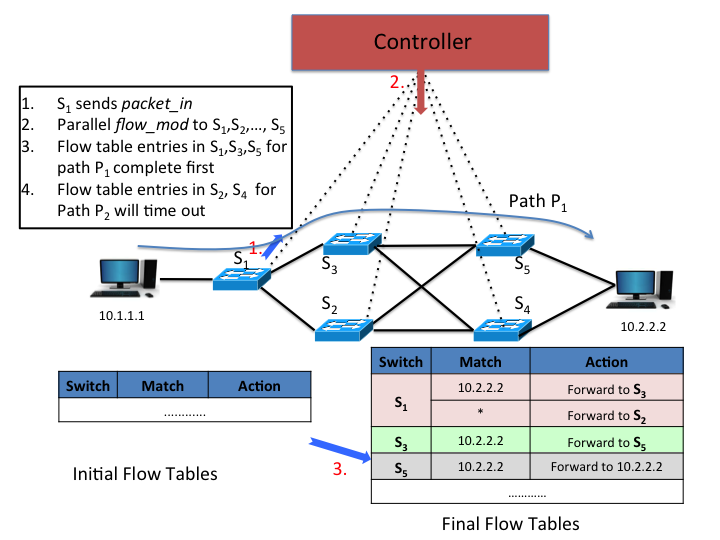
\includegraphics[width=3.5in]{figs/Mazu-mpath.png}
\caption{Exploiting parallel path setup}
\label{fig:mpath}
\end{figure}
%At the lowest level, Broadcom's SDK writes entries to specific addresses in the
%TCAM. If there are multiple entries, the one at the lower address always
%wins. But when you insert a single entry, the Broadcom SDK has no idea whether
%most of the entries you will insert later will be higher or lower
%priority. Nevertheless, it needs to pick an address. Whatever it picks it will
%be wrong for some input pattern. The update rates you see will depend on the
%specific heuristics used for picking addresses -- I do not know the
%specifics. The problem is that after inserting a small percentage of the
%entries, you will want to insert a new one between two existing entries, but
%they will be at adjacent addresses. So you have to make room by doing a
%"shuffle". It's no big deal if you only need to move one entry up or down by one
%address to make room, but as the device fills up you may need  to shuffle a
%large percentage of the entries to make room for the newcomer. Neither is it
%possible to game the system and make a lot of room for future entries because
%you don't know where they will need the room. Again, there are heuristics
%governing shuffles and how aggressively and proactively they are done -- I don't
%know the specifics of what they use. 

As we have seen in Figure x, \flowmod\ delay can be significantly affected by
other switch agent activities such as polling flow statistics.
%$flow\_mod$ time can be very preditable if all of
%them have the same priority. This is because no TCAM rule shuffles are needed.
%However, when rules have different priorities, different addresses are
%picked. Depending on the addresses picked, one may need to make room for new
%entries. Thus, shuffling may happen. \aditya{I don't think we want to use this
%  as a motivation because it contradicts what we are doing for flow engineering,
%  where we assume that the impact of priorities is predictable. why not use
%  pollstats and other uncontrolled activity as motivation??}  
%
To deal with unpredictible delay, we try to setup multiple paths. Data plane packets will
flow as soon as one path completes the setup. 
%\aditya{from here on out, the section was very hard to follow}
First, we illustrate our ideas using a simple example in
Figure~\ref{fig:mpath}. In this five-switch toplogy with switch
$S_1$,$S_2$,$\cdots$, $S_5$, host 10.1.1.1 originates a flow to host
10.2.2.2. Initially all flow tables are empty.
%entry that forward traffic to $S_2$. That is, $S_1$ delegates $packet\_in$
%processing to $S_2$. The reason for the delegation approach is to guard again the
%case that it takes sw1 a long time to install the rules. \emph{Essentially, we create
%two parallel paths even if a flow has a single ingress!} 
When sw1 receives the packet from 10.1.1.1, it will perform
the $packet\_in$ function (step 1). This can be done through our middlebox idea or
directly involve $S_1$'s CPU to generate a $packet\_in$ message and send to
controller. 
%The key point to note is that the $packet\_in$ message will have the
%incoming port information. For our middlebox idea, the incoming port ID can be
%stamped in the IPID field of the first packet before label switch it to the
%middlebox. 

%When the controller receives the $packet\_in$ message with the incoming port
%information, it knows that switch $S_2$ is acting as the delegate of switch
%$S_1$. 
In step 2 shown in the figure, the controller will set parallel
$flow\_mod$ messages to install rules for two paths: (1) path 1 is $S_1$,$S_3$,
$S_5$; (2) path 2 (except ingress) is $S_2$, $S_4$. In order for the controller to know
that $flow\_mod$ has appeared in a switch's hardware flow table, the controller
can send barrier messages to switches. Barrier messages request switch to notify
the controller when all rules before the barrier message is installed (not all
switch implement barrier message or implement it with a 
blocking semantics, i.e. barrier reply message is sent after the rule appears in
TCAM).  %\aditya{the sentence in paranthesis does not parse}

There are two cases. Case 1: suppose the controller
receives the barrier reply messages from all switches in path $P_1$ before path
2's $S_2$ and $S_4$. The controller will send a $packet\_out$ message to switch $S_1$. 
%The controller supplies the complete packet in the message. 
The first packet will be routed
through switch $S_3$ and $S_5$ to the destination. Our middlebox idea nicely
handles the case that multiple packets accumulate before the path setup
completes. Switch $S_2$ and $S_4$'s rule entries for path 2 will be timed out
since no traffic will follow. Case 2: path $P_2$'s $S_2$, $S_4$ comes back
first. Suppose $S_1$ also comes back. Then the controller will modify the rule
entry so that the action will direct traffic to path 2.   
% However, when the entry for 10.2.2.2 appears in $S_1$'s hardware flow
%table. Packets will match this high priority rule. So the flow from 10.1.1.1 to
%10.2.2.2 will experience a path switching. If we pick the two paths with similar
%latency, packet reordering should be easily handled at the destination. After
%the switching, rule entries at sw2 and sw4 will be timed out.

\program{prog:mflow-mpath}
    {Parallel Path Setup for Multiple Flows}
{
//$N$ flows, compute $K$ disjoint paths per flow \\
//$maxNEntries$: maximal additional entries we place in each switch \\
while ($i<K$) \{ \\
\> while ($j<N$) \{ \\
\>\>ComputeDisjointPath($flow_j$, $i$) //prune switches belong to more than \\
\>\>\> $maxNEntries$ paths \\
\>\>    $j = j+1$ \\
\> \} \\    
\> $i=i+1$ \\
}

Now we describe an algorithm that can work with concurrent setups of many
flows and each flow can have $K$ paths. For a target application such as
mobility, each UE demands a path with low data plane latency. Instead of
computing one shortest path (in terms of latency), we compute $K$ disjoint
shortest paths or $K$ paths such that each switch belongs to at most $L$ paths,
$L<K$. For simplicity, we consider the former. This problem is NP-hard. We can
take any known good approximation algorithm. We can concurrently setup these
$K$ paths in parallel as in our example. 

For joint solution of multiple flows, we will impose a constraint that no
switch should handle more than $MaxNEntries$ number of $flow\_mod$.  For
fairness, we compute one path for all flows before computing the second
joint path for all flow and so on.  The algorithm is shown in
Figure~\ref{prog:mflow-mpath}. 

%\li{add the algorithm pseudo code}

\iffalse
For mobility, we can compute K-paths per flow or jointly. (1) For per flow, lets
use K shortest paths (i.e. ECMP). These K paths should be disjoint or share
minimal number of switches. Lets use disjoint paths. (2) For joint solution of
multiple flows, we will have the same MaxNEntries constraint per switch. For
fairness, you can compute one path for all flows before computing the second
joint path for all flow, etc.  


Even while I was at Broadcom I had little visibility into how the switch guys'
software handled their TCAM. Now that I'm outside I have zero visibility (I work
on search, not on network infrastructure at Google). But I have a broad
explanation of what you see that I am pretty confident is correct. 
 
The API allows you to associate priorities with rules/entries. The API does not
let you tell the hardware how many lower priority or higher priority rules you
will insert in the future. Nor is this easy to figure out, so even if there were
such API, it would be hard to use. But this is exactly what the software would
need in order to ensure fast updates. A more realistic alternative API would be
to give all the entries at once - I don't know whether such a batch API is
available. 

At the lowest level, Broadcom's SDK writes entries to specific addresses in the
TCAM. If there are multiple entries, the one at the lower address always
wins. But when you insert a single entry, the Broadcom SDK has no idea whether
most of the entries you will insert later will be higher or lower
priority. Nevertheless, it needs to pick an address. Whatever it picks it will
be wrong for some input pattern. The update rates you see will depend on the
specific heuristics used for picking addresses -- I do not know the
specifics. The problem is that after inserting a small percentage of the
entries, you will want to insert a new one between two existing entries, but
they will be at adjacent addresses. So you have to make room by doing a
"shuffle". It's no big deal if you only need to move one entry up or down by one
address to make room, but as the device fills up you may need  to shuffle a
large percentage of the entries to make room for the newcomer. Neither is it
possible to game the system and make a lot of room for future entries because
you don't know where they will need the room. Again, there are heuristics
governing shuffles and how aggressively and proactively they are done -- I don't
know the specifics of what they use. 

One common property of all these TCAM shuffle algorithms is that they work
spectacularly well when entries have the same priority. Shuffles are not
needed. The Broadcom SDK is allowed to write the new entries to any available
TCAM address. 

Please let me know if anything you see contradicts this explanation - there may
be more going on, but usually the shuffles are the big update rate killer. 

Cheers,

Cristi



On Tue, Jan 21, 2014 at 12:59 PM, Aditya Akella <akella@cs.wisc.edu> wrote:
Hi Cristi,

One other question for you that has really been bugging us and we simple can't figure out what's going on. We did a bunch of experiments where we see bizarre and inconsistent results.

Expt 1: We conducted an experiment where we installed a burst of rules of size B of a certain priority pattern P. We measure total latency to install the rules:

1. B --> increasing priority: we see latencies really shoot up, with the burst taking almost 30s to install. This makes sense as perhaps each incoming higher priority rule is causing TCAM rearrangement (?)
2. B --> decreasing priority: we see high latencies too, over 20s to install. We did not expect this as we were hoping the latencies would be the same as B --> same priority.

Any thoughts on what may be going on? So we thought something weird is happening with low/high priorities, so we decided to run a bunch of experiments that played with the pattern of priorities. Here are a couple:

Expt 2: We installed ~700 each of alternating high and low priorities. We saw all rules with the higher priority were installed first (within ~1.5s in all) after which the low priority rules started to get inserted, which kind of makes sense except that the  low latency rule installation completed after 20s or more!

But:

Expt 3: If instead of sending the burst of about 700 above, we first sent 350 high priority rules, and then send a burst of 350 low priority rules after the first batch was installed, then the completion time of the latter is far far lower than what we see in Expt 2.

What on earth is going on? Can you shed some light in general on how Broadcom handles priorities? Is there some obvious issue we are missing out on?

\fi

\subsection{Rule Reordering}
\label{s:optimal}

Our measurements show that given rules of different priorities to be inserted at
a switch, the ``optimal'' order of rule insertion varies with switch platform
because of the difference in architecture and the workload the hardware is
optimized for. For Intel, the optimal order is to insert
rules in \emph{increasing} order of priority, whereas the \emph{opposite} is
true for Broadcom. Given this observation, Mazu controls the actual rule
insertion using the pattern that is optimal for the switch. 

We assume one-shot consistent updates~\cite{one-shot} are in use. In this case, new rules will not take effect unless all of them are installed. Therefore, Mazu can optimize the ordering without causing temporal policy violations. Mazu's techniques can also be adapted for other update schemes~\cite{mahajan13:hotnets}.

%\aditya{is there more to say here?} 

% \aditya{I'm not sure what our measurements show here. Is a particular insertion order better than another?}

% \aditya{Li and I were thinking that given a set of rules to insert into a switch, the idea would be to sort them in descending order of priority and insert. The intuition is that the higher priority rules inserted earlier will not be disturbed by later lower priority rules (in contrast if we change the order then a lower priority rule inserted earlier may have to be moved around to make room for a later higher priority rule).
% However, our experiments are inconclusive in this respect, correct? (we see that decreasing priority order has somewhat arbitrary performance, and shows abnormally high latency? Also when we interleave priorities we see all high priority inserted first.)
% So what is our story here?}

% LocalWords:  Broadcom Mazu


% LocalWords:  TCAMs OpenFlow SDK ACLs Mazu Broadcom
